\section*{Anexos}
\addcontentsline{toc}{section}{Anexos}

\begin{figure}[h]
    \centering
    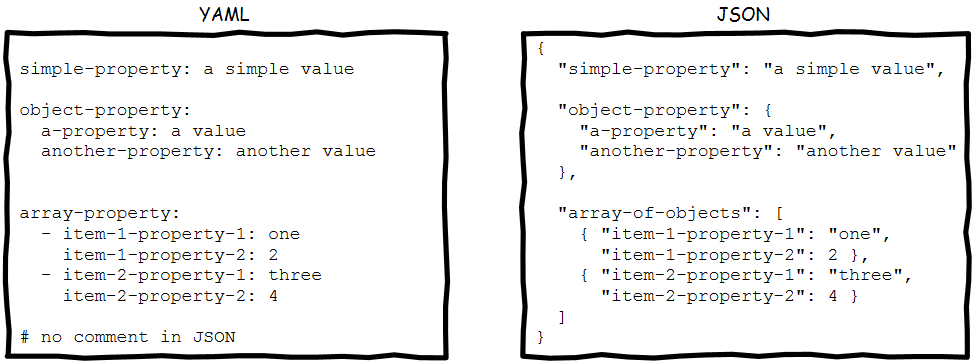
\includegraphics[width=\linewidth]{images/yaml-vs-json.png}
    \caption{Comparación de sintaxis entre YAML y JSON}
    \label{fig:yaml-vs-json}
\end{figure}

\begin{figure}[h]
    \centering
    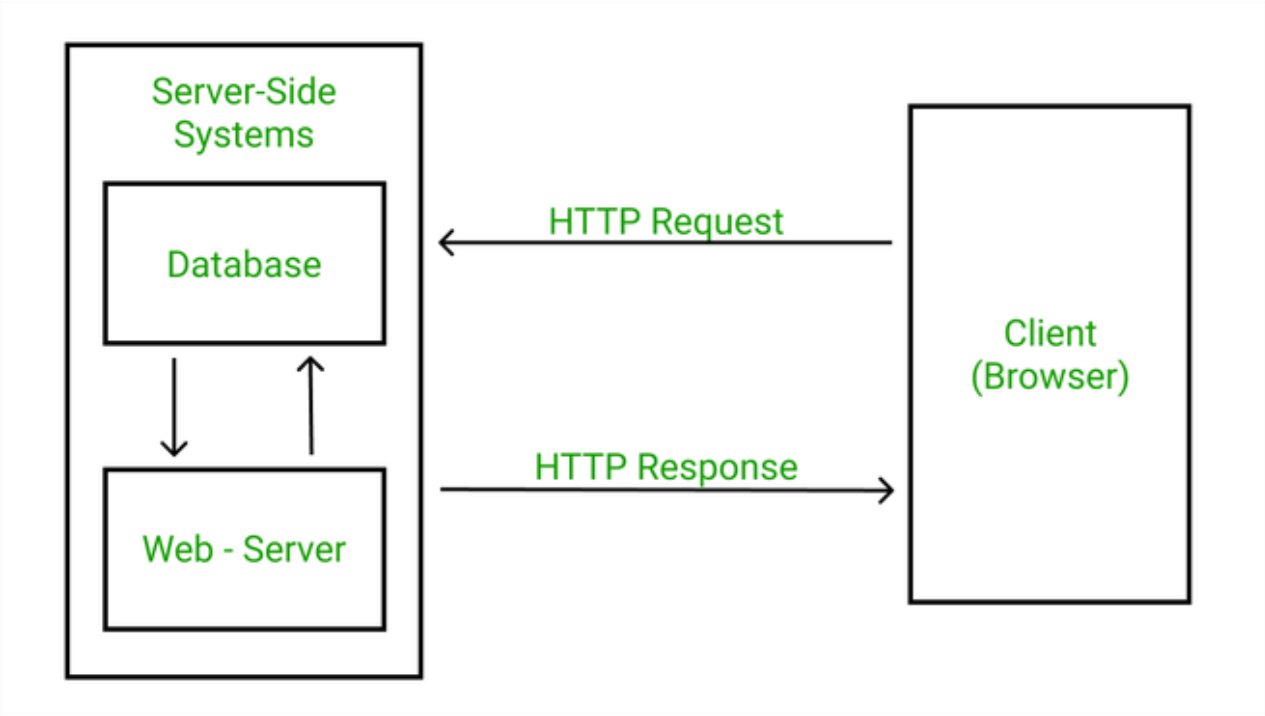
\includegraphics[width=\linewidth]{images/call-return-style.png}
    \caption{Diagrama representando el estilo arquitectónico Llamada Retorno}
    \label{fig:call-return-style}
\end{figure}

\begin{figure}[h]
    \centering
    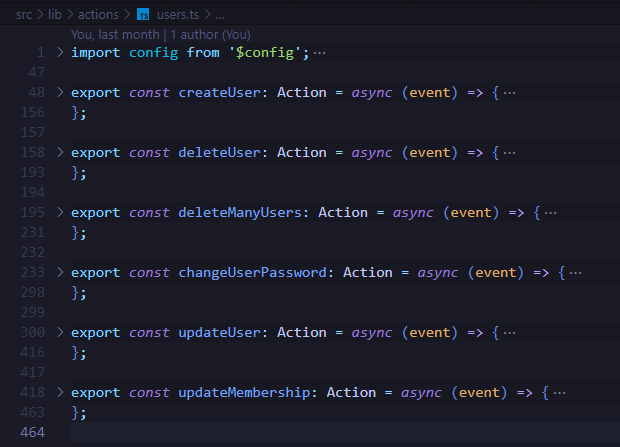
\includegraphics[scale=0.8]{images/code/collapsed-view-of-user-module.png}
    \caption{Vista colapsada del módulo de encargado de la gestión de usuarios}
    \label{fig:collapsed-view-of-user-module}
\end{figure}

\begin{figure}[h]
    \centering
    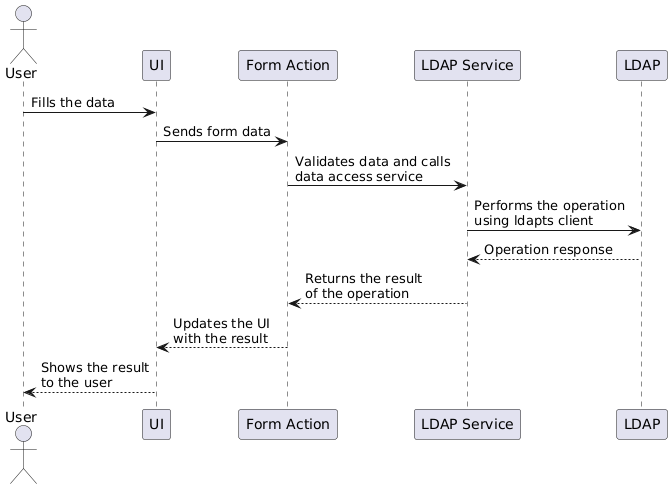
\includegraphics[width=\linewidth]{images/puml/sequence diagram form submission/sequence diagram form submission.png}
    \caption{Diagrama de sequencia mostrando un flujo de envío de formulario general}
    \label{fig:general-form-submission-diagram}
\end{figure}

\newpage
\begin{figure}[h]
    \centering
    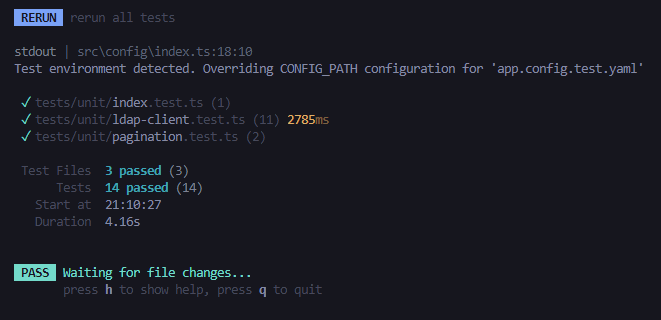
\includegraphics[width=\linewidth]{images/vitest tests run successfully.png}
    \caption{Pruebas con vitest pasaron exitosamente}
    \label{fig:integration-tests-run-ok}
\end{figure}

\begin{figure}[h]
    \centering
    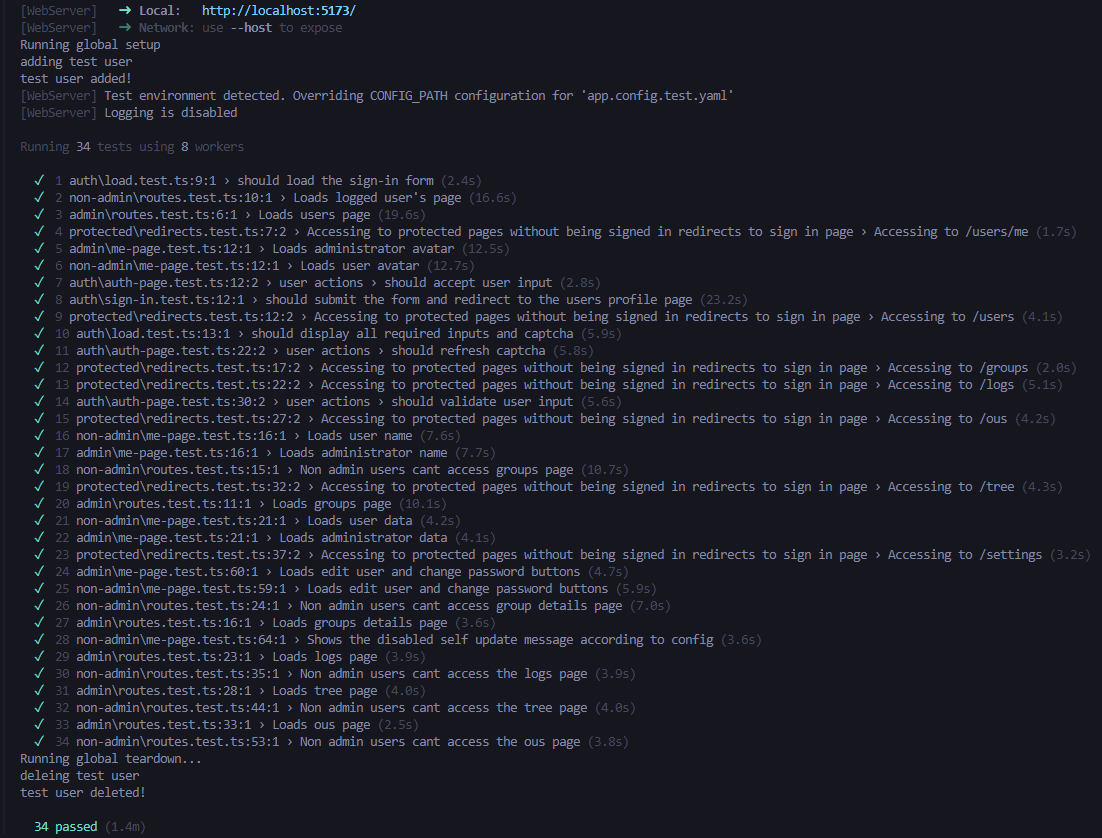
\includegraphics[width=\linewidth]{images/playwright tests run successfully.png}
    \caption{Pruebas de e2e pasaron exitosamente}
    \label{fig:e2e-test-run-ok}
\end{figure}


\begin{figure}[h]
    \centering
    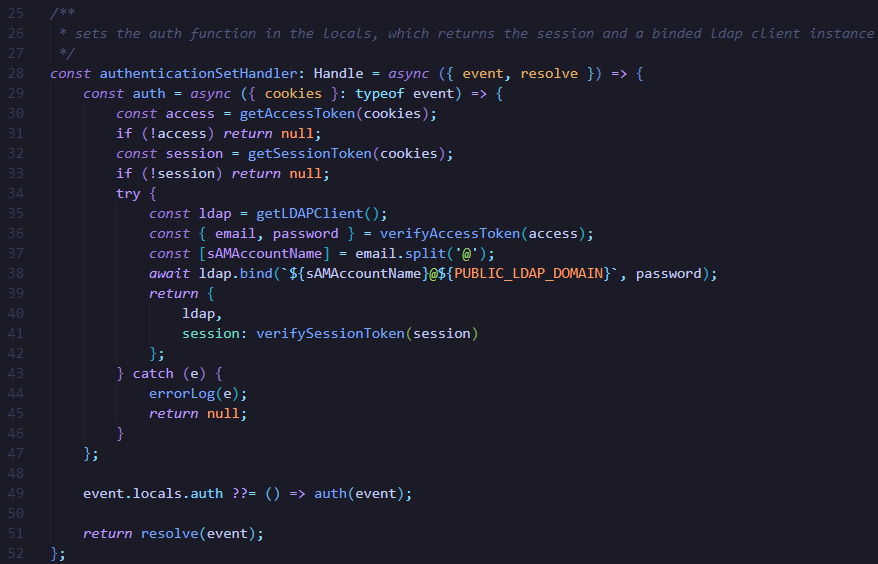
\includegraphics[width=\textwidth]{images/code/authenticationSetHandler.png}
    \caption{Manejador: autenticación y creacion del cliente LDAP}
    \label{fig:authentication-set-handler}
\end{figure}

\begin{figure}[h]
    \centering
    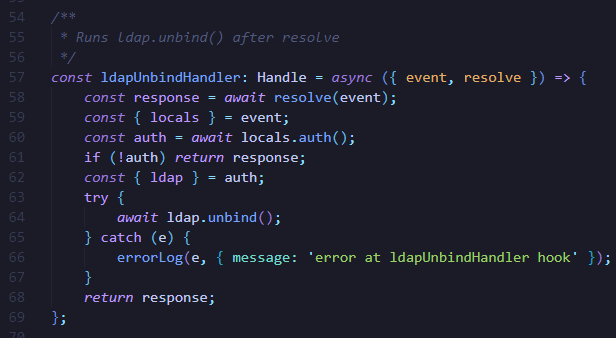
\includegraphics[width=\textwidth]{images/code/ldapUnbindHandler.png}
    \caption{Manejador: Cierre de la conexion del cliente LDAP}
    \label{fig:ldap-unbind-handler}
\end{figure}


\newgeometry{hmargin=0.5cm, vmargin=3cm}
\begin{figure}[h]
    \centering
    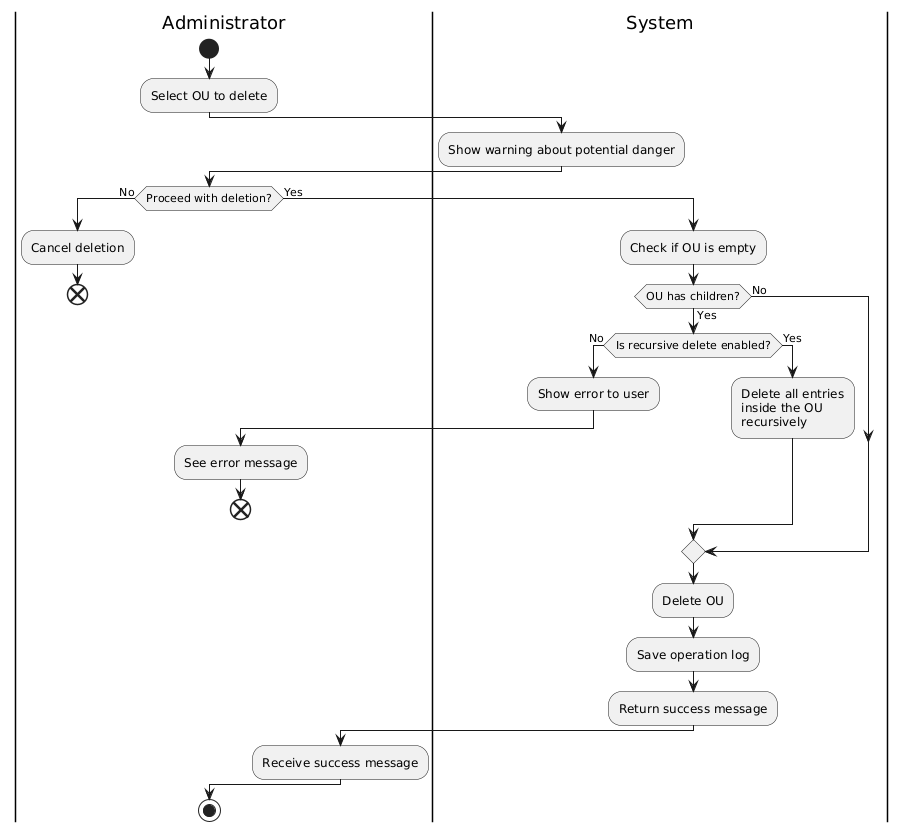
\includegraphics[width=\linewidth]{images/puml/activity-diagram delete ou/activity-diagram delete ou.png}
    \caption{Diagrama de actividades: Eliminar Unidad Organizacional}
    \label{fig:activity-diagram-delete-ou}
\end{figure}
\restoregeometry

\newpage
\newgeometry{hmargin=1cm, vmargin=3.5cm}
\begin{landscape}
    \begin{figure}
        \centering
        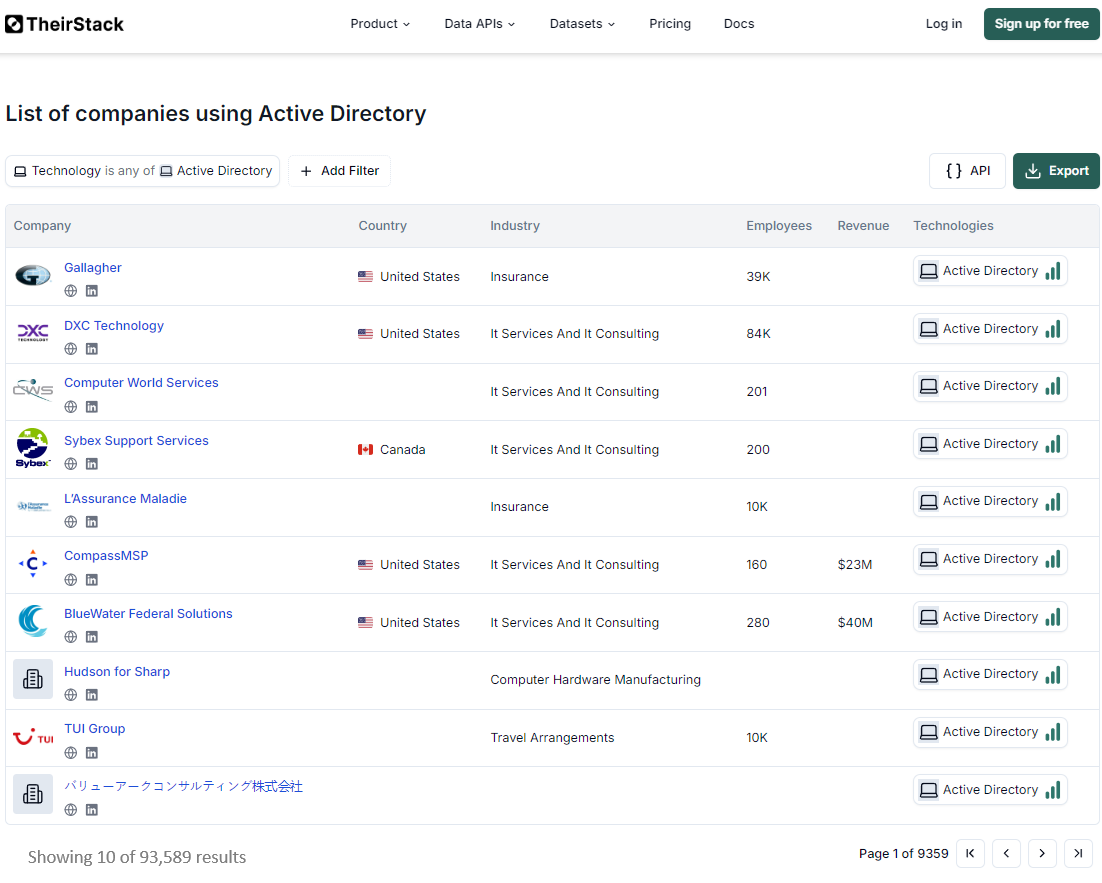
\includegraphics[width=\linewidth]{images/companies using ad - 2 .png}
        \caption{Compañías que usan Directorio Activo hoy en dia en el mundo (90 000+)}
        \label{fig:companies-using-ad}
    \end{figure}

    \begin{figure}[h]
        \centering
        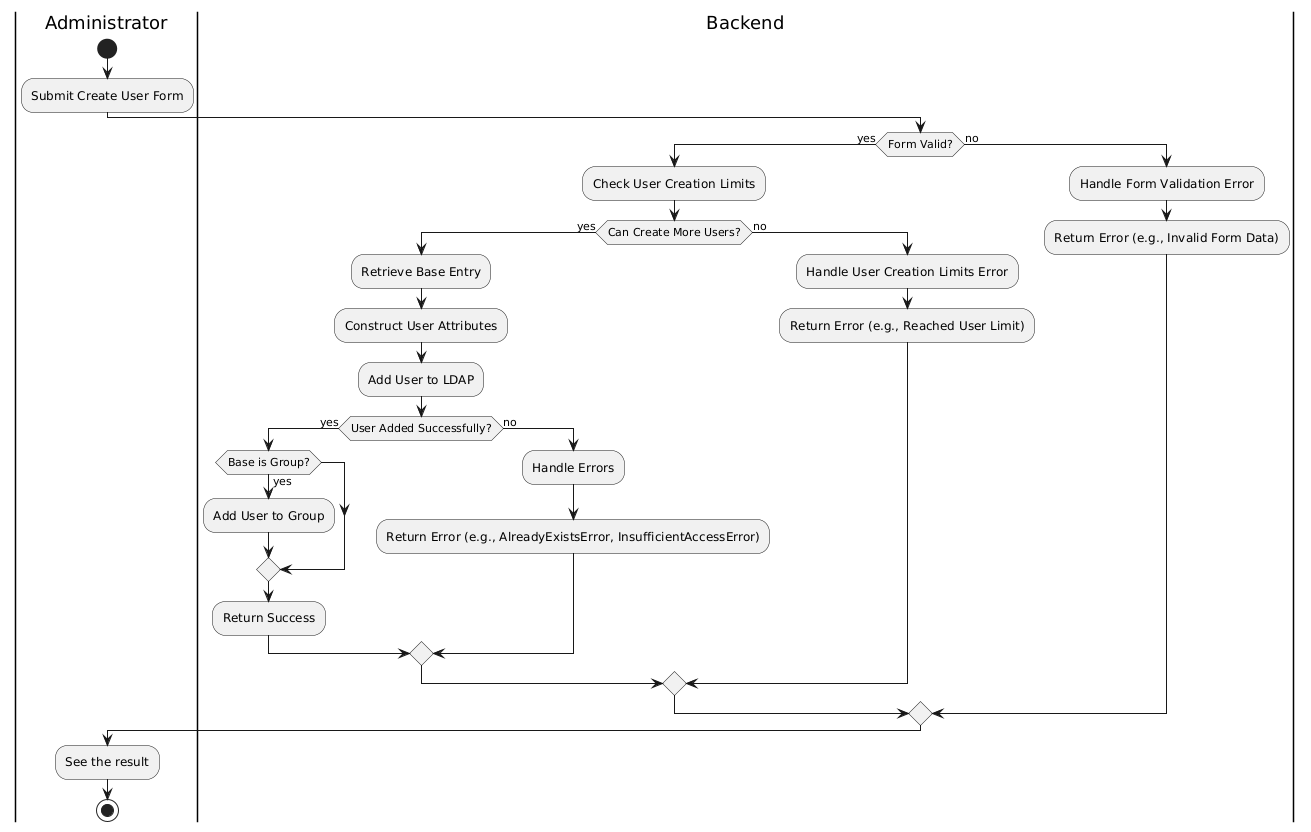
\includegraphics[scale=0.55]{images/puml/activity-diagram-create-user/activity-diagram create user.png}
        \caption{Diagrama de actividades: Crear usuario}
        \label{fig:activity-diagram-create-user}
    \end{figure}
\end{landscape}
\restoregeometry


\newgeometry{vmargin=1.5cm}
\begin{figure}[h]
    \centering
    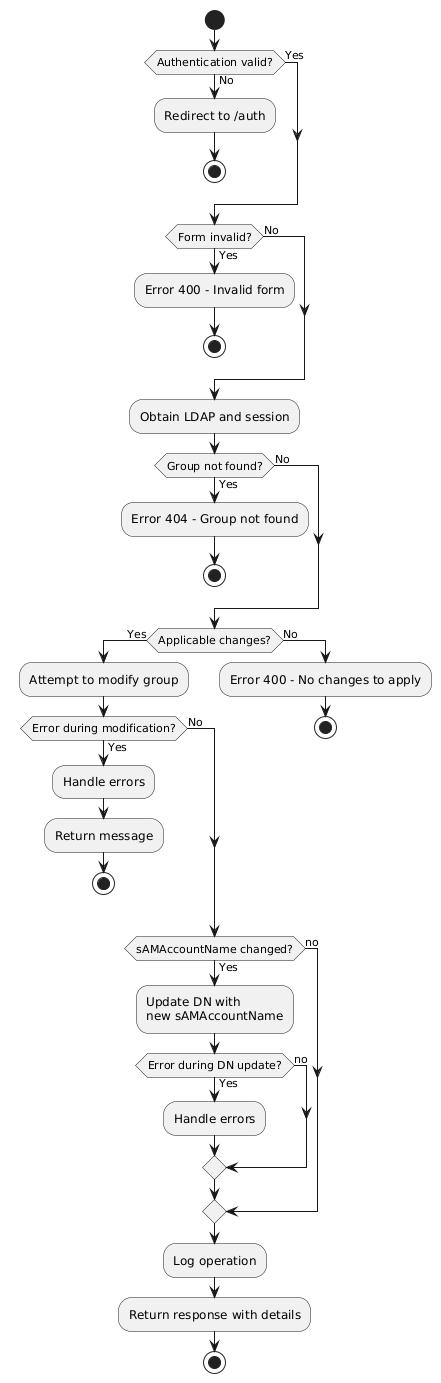
\includegraphics[height=26cm]{images/puml/flow-diagram-update group/flow-diagram update group.png}
    \caption{Diagrama de flujo: Actualizar grupo}
    \label{fig:flow-diagram-update-group}
\end{figure}
\restoregeometry